\documentclass{llncs}
\usepackage[utf8]{inputenc}
\usepackage{graphicx}
%\usepackage{listings}

% set PDF to version 5 as some included images use 1.5
\pdfoptionpdfminorversion=5

\begin{document}
\title{Transformation As Search}
\author{Mathias Kleiner\inst{2} \and Marcos Didonet Del Fabro\inst{1} \and Davi De Queiroz Santos\inst{1}}

\institute{ 
C3SL labs; Depto. de Informatica\\Universidade Federal do Parana', Curitiba, PR, Brazil \\
\email{marcos.ddf,daqsantos@inf.ufpr.br}
\and
Arts et Métiers ParisTech ; CNRS, LSIS, 2 cours des Arts et
Métiers, 13697 Aix-en-Provence, France\\
\email{mathias.kleiner@ensam.eu}
}

\maketitle

\begin{abstract}
In model-driven engineering, model transformations are considered a key element
to generate and maintain consistency between related models. Rule-based
approaches have become a mature technology and are widely used in different application
domains. However, in various scenarios, these solutions still suffer from a
number of limitations that stem from their injective and deterministic nature. This
article proposes an original approach, based on non-deterministic constraint-based search engines, 
to define and execute bidirectional model transformations and synchronizations from single specifications. Since these solely rely on basic existing modeling concepts, it does not require the introduction of a dedicated language. We first describe and formally define this model operation, called \emph{transformation as search}, then describe a proof-of-concept implementation and discuss experiments on a reference use case in software engineering.
\end{abstract}
%
\setcounter{tocdepth}{2}
%\tableofcontents
%
\section{Introduction}

In existing Model-driven Engineering (MDE) approaches, model transformations are
a key element for performing operations between different models. These operations
may be of different nature, such as migration, evolution, composition, exchange,
and others. 
Despite the existing solutions being very different on the set of
available capabilities (see \cite{czarnecki} for a survey), most of them are rule-based approaches.

These approaches have a simple and efficient principle: given a source metamodel $MMa$ and a
target metamodel $MMb$, the developer defines a set of pattern-matching rules to transform all the model elements from $MMa$ into elements of $MMb$. These transformation engines have a deterministic behavior,
i.e., one source model always produces the same target model. In addition, the
transformation rules  are unidirectional and need to be fully-specified, i.e., it is necessary to
write rules that cover all the (relevant) elements of $MMb$.

These properties limit the scope of most transformation languages in various scenarios \cite{DBLP:conf/icmt/CzarneckiFHLST09}. For instance it may be hard to write rules that cover all the transformation cases. Similarly, it is sometimes desirable to produce more than one target model in order to study the alternatives. Bidirectional behavior requires to write or derive a reverse transformation. Finally, these approaches hardly allow to maintain models consistency without additional mechanisms.

Some of these limitations are directly linked to the fact that most tools do not allow
for disjunctions (i.e., choice points in the sense of combinatorial problems) and take decisions solely on the basis of
the source model. Indeed searching for multiple target models requires non-deterministic
properties: a given source model may produce zero, one or multiple target models
that satisfy a set of constraints.

In this paper, we present a novel approach that uses constraint-based search for
executing model transformations and synchronizations. At this stage, our challenge is to present this approach to
the community and to integrate it at its best in current MDE 
practices. To this aim, we reuse and extend a \emph{model search} operation proposed in previous work\cite{modelsearch09} as well as its notion of {\it partial} model: a model whose known constituents actually conform to their corresponding metamodel, but that should be interpreted with a weaker conformance than the classical closed-world interpretation used in the MDE community.

The core idea is to create a unified metamodel containing source, transformation and target constraints. Different scenarios (creation of target model(s), synchronization of existing models, and others) then mainly resolve to searching for conforming model(s).  
First, we define a (potentially partial) set of correspondences (i.e., transformation constraints) between the source and target
metamodels using basic modeling concepts. Second, we transform the input artifacts into a solver which executes the scenario through a generic model search operation. As a result the engine produces none, one or several output models that \emph{contain} the 
solution(s) and its generation traces. The specifications are
bi-directional and flexible: they can be used to produce either the source or the target
model, or even propagate changes from one model to the other depending on the chosen scenario. 
Another interesting property is that one could introduce an
optimization criterion that will be used by the search process to produce one
specific solution (the ``best'' one). 
%
\paragraph{Plan of the article}
%
Section \ref{sec:context} briefly introduces the context of model-driven
engineering, constraint programming main principles, and recalls necessary
definitions from previous work on \emph{model search}. 
Section \ref{sec:TAS} formally defines the \emph{transformation as search} operation, and describes a generic process for its realization along with a running example. Section \ref{sec:validation} proposes a prototype implementation and discusses preliminary experiments on a reference use case. Finally, Section \ref{sec:rfwork} discusses related work and Section \ref{sec:conclusion} concludes.
%
\section{Context}
\label{sec:context}
\subsection{Introduction to MDE and model transformation}
Model Driven Engineering considers models, through multiple abstract
representation levels, as a unifying concept. The central concepts that have been
introduced are terminal model, metamodel, and metametamodel. A terminal model is
a representation of a system. It captures some characteristics of the system and
provides knowledge about it. MDE tools act on models expressed in
precise modeling languages. The abstract syntax of a modeling language, when
expressed as a model, is called a metamodel. The relation between a model and the
metamodel of its language is called $conformsTo$. Metamodels are in turn
expressed in a modeling language for which conceptual foundations are captured in
an auto-descriptive model called metametamodel. The main way to automate MDE is
by executing operations on models. For instance, the production of a model $Mb$
from a model $Ma$ by a transformation $Mt$ is called a model transformation. The
OMG's Query View Transform (QVT) \cite{QVT} defines a set of useful model
operations languages. In particular, it defines a language called QVT-operational which is restricted to unidirectional transformations scenarios, and a language called QVT-relational which can be used for bidirectional and synchronization scenarios. 
%
There are multiple model definitions in the literature (see \cite{DBLP:journals/sosym/Kuhne06} for a deep study), we refine in this article the
ones introduced in \cite{DBLP:conf/fmoods/JouaultB06}\footnote{Though these may not be the most precise on object-oriented concepts and different model relationships, simple graph-based definition will prove useful in our context}.

\begin{definition} [model] A model M is a triple $<G, \omega,
\mu>$ where:
\begin{itemize}
\item G is a directed labelled multigraph,
\item $\omega$ (called the reference model of M) is either another model or M itself (i.e., self-reference)
\item $\mu$ is a function associating nodes and edges of G to nodes of $G_\omega$ (the graph associated to its reference model $\omega$)
\end{itemize}
\end{definition}
%
\begin{definition}[conformance] The relation between a model and its reference model is called conformance and noted $conformsTo$.
\end{definition}
%
\begin{definition}[metametamodel] A metametamodel is a model that is its own
reference model (i.e., it $conformsTo$ itself).
\end{definition}
\begin{definition}[metamodel] A metamodel is a model such that its reference
model is a metametamodel.
\end{definition}
\begin{definition}[terminal model] A terminal model is a model such that its
reference model is a metamodel.
\end{definition}
%
\subsection{Constrained metamodels}
%
The notion of constraints is closely coupled to MDE. Engineers have been using
constraints to complete the definition of metamodels for a long time, as
illustrated by the popular combination UML/OCL \cite{OCL-spec}. Constraints can be, for instance,
checked against one given model in order to validate it. In our approach we
will always consider metamodels with potential constraints attached. We
refine in this article definitions from \cite{modelsearch09} to formally define
the combination: 

\begin{definition}[constrained metamodel] A constrained metamodel $CMM$ is a pair $<MM, C>$ where $MM$ is
a metamodel and $C$ is a set (a conjunction) of predicates over elements of the
graph $G$ associated to $MM$. We will consider an oracle that, given a model $M$,
returns true (noted $M \in C(MM)$ where $C(MM)$ is the set of all valid models) iff $M$ satisfies all  predicates from $C$.
\end{definition}
%
The conformance relation between a model and its reference is then naturally extended to constrained metamodels.
%
\begin{definition}[constrained conformance]\label{def:conformance} A model $M$ \emph{conformsTo} a constrained metamodel $CMM$ iff it $conformsTo$ $MM$ and $M \in C(MM)$.
\end{definition}
Many languages can be used to define predicates (i.e., constraints) with
different levels of expressiveness. OCL supports operators on sets and relations
as well as quantifiers (universal and existential) and iterators. To ease the specification of metamodel static constraints, we use in this article an OCL-compatible extension (OCL+ \cite{ICFG-MM-usecase}) that extends it with multi-context constraints.
%
\subsection{Introduction to constraint programming}
\label{sec:cp}
Constraint programming (CP) is a declarative programming technique to solve
combinatorial (usually NP-hard) problems. A constraint, in its wider sense, is a
predicate on elements (represented by variables). A CP problem is thus defined by
a set of elements and a set of constraints. The objective of a CP solver is to
find an assignment (i.e, a set of values for the variables) that satisfy all the
constraints. There are several CP formalisms and techniques
\cite{DBLP:journals/jlp/JaffarM94} which differ by their expressiveness,
the abstractness of the language and the solving algorithms.
\subsection{Introduction to model search}
\label{sec:ms}
A solver-independent integration of constraint programming, called \emph{model
search}, for the automatic generation (or completion) of constrained models has been described in
\cite{modelsearch09}. This article builds on those foundations to propose a generic
model transformation method based on constrained search. Therefore we need to briefly recall here
the main principles and definitions of the model search operation.\\
\begin{definition}[relaxed metamodel]\label{def:relaxed-metamodel} Let
$CMM=<MM,C>$ (with $MM=<G, \omega,
\mu>$) be a constrained metamodel. $CMM_r=<MM_r,C_r>$ (with $MM_r=<G_r, \omega,
\mu>$) is a relaxed metamodel of CMM (noted $CMM_r \in
Rx(CMM)$) if and only if $G_{MM_r} \subseteq G_{MM}$ and $C_r \subseteq C$.
\end{definition}
In other words, a relaxed metamodel is a less constrained (and/or smaller) metamodel. A simple one can be obtained by the removal of all constraints. Computing such a relaxed
metamodel, a simple operation which can obviously be done easily with existing techniques, is called \emph{relaxation} in the following.
\begin{definition}[partial model, p-conformsTo] \label{def:partial-model} Let
$CMM=<MM,C>$ be a constrained metamodel and $M_r$ a model. $M_r$ $p$-$conformsTo$ $CMM$ iff it conforms to a
metamodel $CMM_r$ such that $CMM_r$ is a relaxed metamodel of $CMM$ ($CMM_r \in
Rx(CMM)$). $M_r$ is called a partial model of $CMM$.
\end{definition}
Informally, a partial model is simply understood as being an incomplete model.
\begin{definition}[model search]\label{def:model-search} Let $CMM=<MM,C>$ be a
constrained metamodel, and $M_r=<G_r, MM_r, \mu_r>$ a partial model of $CMM$. Model search is the operation
of finding a (finite) model $M=<G, MM, \mu>$ such that $G_r \subseteq G$, $\mu_r
\subseteq \mu$ (embedding i.e, $\forall x \in Gr, \mu(x) = \mu_r(x))$, and $M$
$conformsTo$ $CMM$.
\end{definition}
In other words, model search extends a partial model into a ``full'' model conforming to its constrained metamodel (or generates one when an empty request $M_r$ is given).
\begin{figure}[htb] \centering 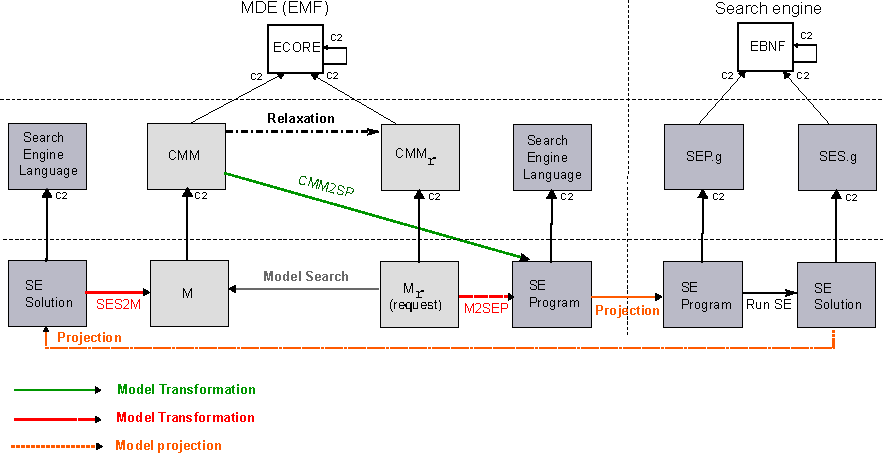
\includegraphics[scale=0.8]{img/SearchMethodology-emf-SearchEngine-smaller-simpler-lighter.pdf}
\caption{Model search: example process}
\label{fig:ModelSearch}
\end{figure}
%
An example process to achieve this operation in a MDE framework is illustrated in Figure \ref{fig:ModelSearch}. Briefly, the request $M_r$ and the metamodel $CMM$ are transformed into the search engine input format where search takes place. The solutions, if any, are then transformed back into the modelling paradigm.\\
We may thus consider model search as a model transformation where the source (metamodel and model) is
an instance of a non-deterministic (combinatorial) problem and the target model
is a solution (if any exists). From the CP point of view, the target metamodel
acts as the constraint model whereas the source model (the request) is a given
partial assignment that needs to be extended.\\
For deeper information on how this operation is formalized, achieved and integrated as a
first-class MDE operation, the reader is kindly referred to \cite{modelsearch09}.
%
\section{Transformation As Search}
\label{sec:TAS}
%
The following proposes to generalize model search to constraint-based model
transformation/synchronization by considering different source and target metamodels. The main
idea is to define the transformation/synchronization as a set of relations and constraints
between elements of the metamodels that are to be related (these may be called \emph{weaving
links}). All these artifacts are then unified into a \emph{transformation metamodel}. By applying model search on this unified metamodel, a model which \emph{contains} valid solution model(s) is created.\\
In the following, we first introduce a running example of a classic transformation scenario (creation of a single target model out of a single source model) which is then used to illustrate the generic process. Its adaptation to other scenarios is then briefly discussed.
%
\subsection{Running example}
%
The chosen use case is a transformation of a class schema
model ($MM^A$) into a relational schema model ($MM^B$), known as the
\textit{Class2Relational} transformation. This use case is well-known due to its
large applicability and it has been studied in other works to demonstrate
different aspects about transformation languages, such as 
\cite{QVT}, \cite{tefkat}, and others. The initial metamodels are
extracted from the public transformation repository at \cite{atlc2r} and illustrated at both sides of Figure
\ref{fig:classAndRelational} (some elements have been omitted to improve readability).\\
The main scenario, which process is described in the following is the creation of a target model (a relational schema) from a source model (a class schema).
%
\begin{figure}[htb] \centering 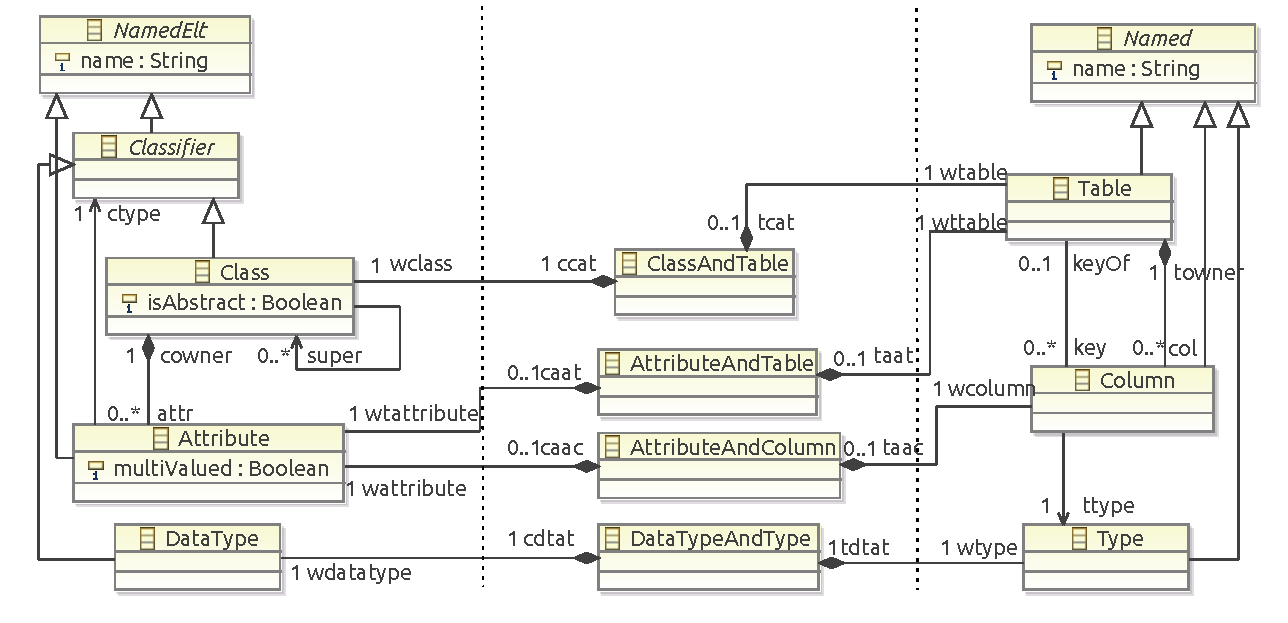
\includegraphics[scale=0.6]{img/CLAR-transformation-metamodel-v1.pdf}
\caption{Extract of the running example transformation metamodel (V1) as an ecore diagram. Initial metamodels are on the sides, weaving metamodel is in the middle.}
\label{fig:classAndRelational}
\end{figure}
%
\subsection{Process}
%
\subsubsection{Obtaining the transformation metamodel by unification}
\begin{figure}[htb]
 \begin{center}
     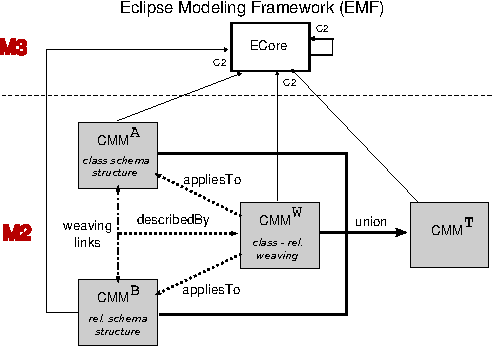
\includegraphics[scale=1.0]{img/CMMT-creation-with_example-lighter.pdf}
\caption{Obtaining the transformation metamodel by unification (application on the running example shown in italics)}
   \label{fig:CMMT-unification}
 \end{center}
\end{figure}
%
Figure \ref{fig:CMMT-unification} shows how to obtain a
transformation metamodel, called $CMM^T$, by unification of the source ($CMM^A$), target ($CMM^B$) and weaving ($CMM^W$) metamodels. In our example these inputs are respectively the class schema structure (left part of Figure \ref{fig:classAndRelational}), the relational schema structure (right part), and a set of weaving elements and constraints (middle part, constraints are not shown in the Figure). This operation, consisting merely in copying and combining the sources, can be done with existing transformation techniques. Formal definitions of $CMM^W$ and $CMM^T$ are given below:
%
\begin{definition}[weaving metamodel]\label{def:weaving-metamodel} We call \emph{weaving metamodel} between metamodels $CMM^A$ and $CMM^B$, a constrained metamodel $CMM^W$ defined by $CMM^W = <MM^W,C^W>$, where $MM^W$ and $C^W$ are respectively a set of metamodel elements and constraints that define the weaving relationships between the elements of $CMM^A$ and $CMM^B$ (it requires the use of inter-model references).
\end{definition}
%
\begin{definition}[transformation metamodel]\label{def:transformation-metamodel} We call \emph{transformation metamodel} between metamodels $CMM^A = <MM^A, C^A>$ and $CMM^B = <MM^B, C^B>$, using a weaving metamodel $CMM^W$, a constrained metamodel $CMM^T$ defined by $CMM^T = <MM^T,C^T>$, where $MM^T = MM^A \cup MM^B \cup MM^W$ and $C^T = C^A \cup C^B \cup C^W$.\\
\end{definition}
%
Obviously, unification turns inter-model references in the weaving metamodel into intra-model references in the transformation metamodel.
%
\subsubsection{Searching for a target model}
%
\begin{figure}[htb]
 \begin{center}
     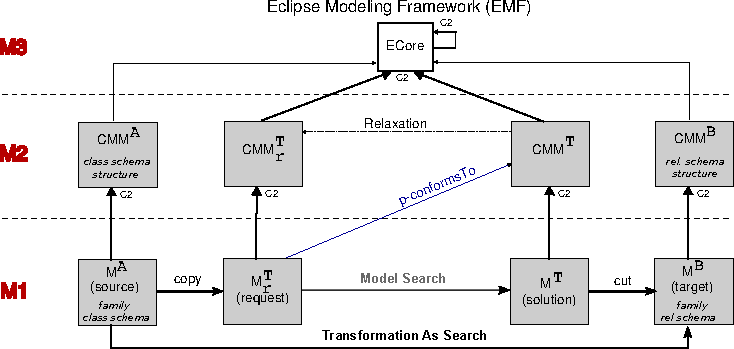
\includegraphics[scale=1.0]{img/TransformationAsSearch-with_example-lighter.pdf}
\caption{Transformation as search operation (application on the running example shown in italics)}
   \label{fig:TransformationAsSearch}
 \end{center}
\end{figure}
%
Figure \ref{fig:TransformationAsSearch} shows how a target model can be created
by applying model search to the transformation metamodel. In this scenario we have
an exogenous unidirectional transformation from one source model ($M^A$) to a target model
($M^B$).\\
%
The first step is to define the model search request. In this
scenario it is simply a copy of the source model. In our running example, it corresponds to the ``Family" class schema at the top of Figure \ref{fig:transformation-result}.
%
\begin{figure}[htb] \centering 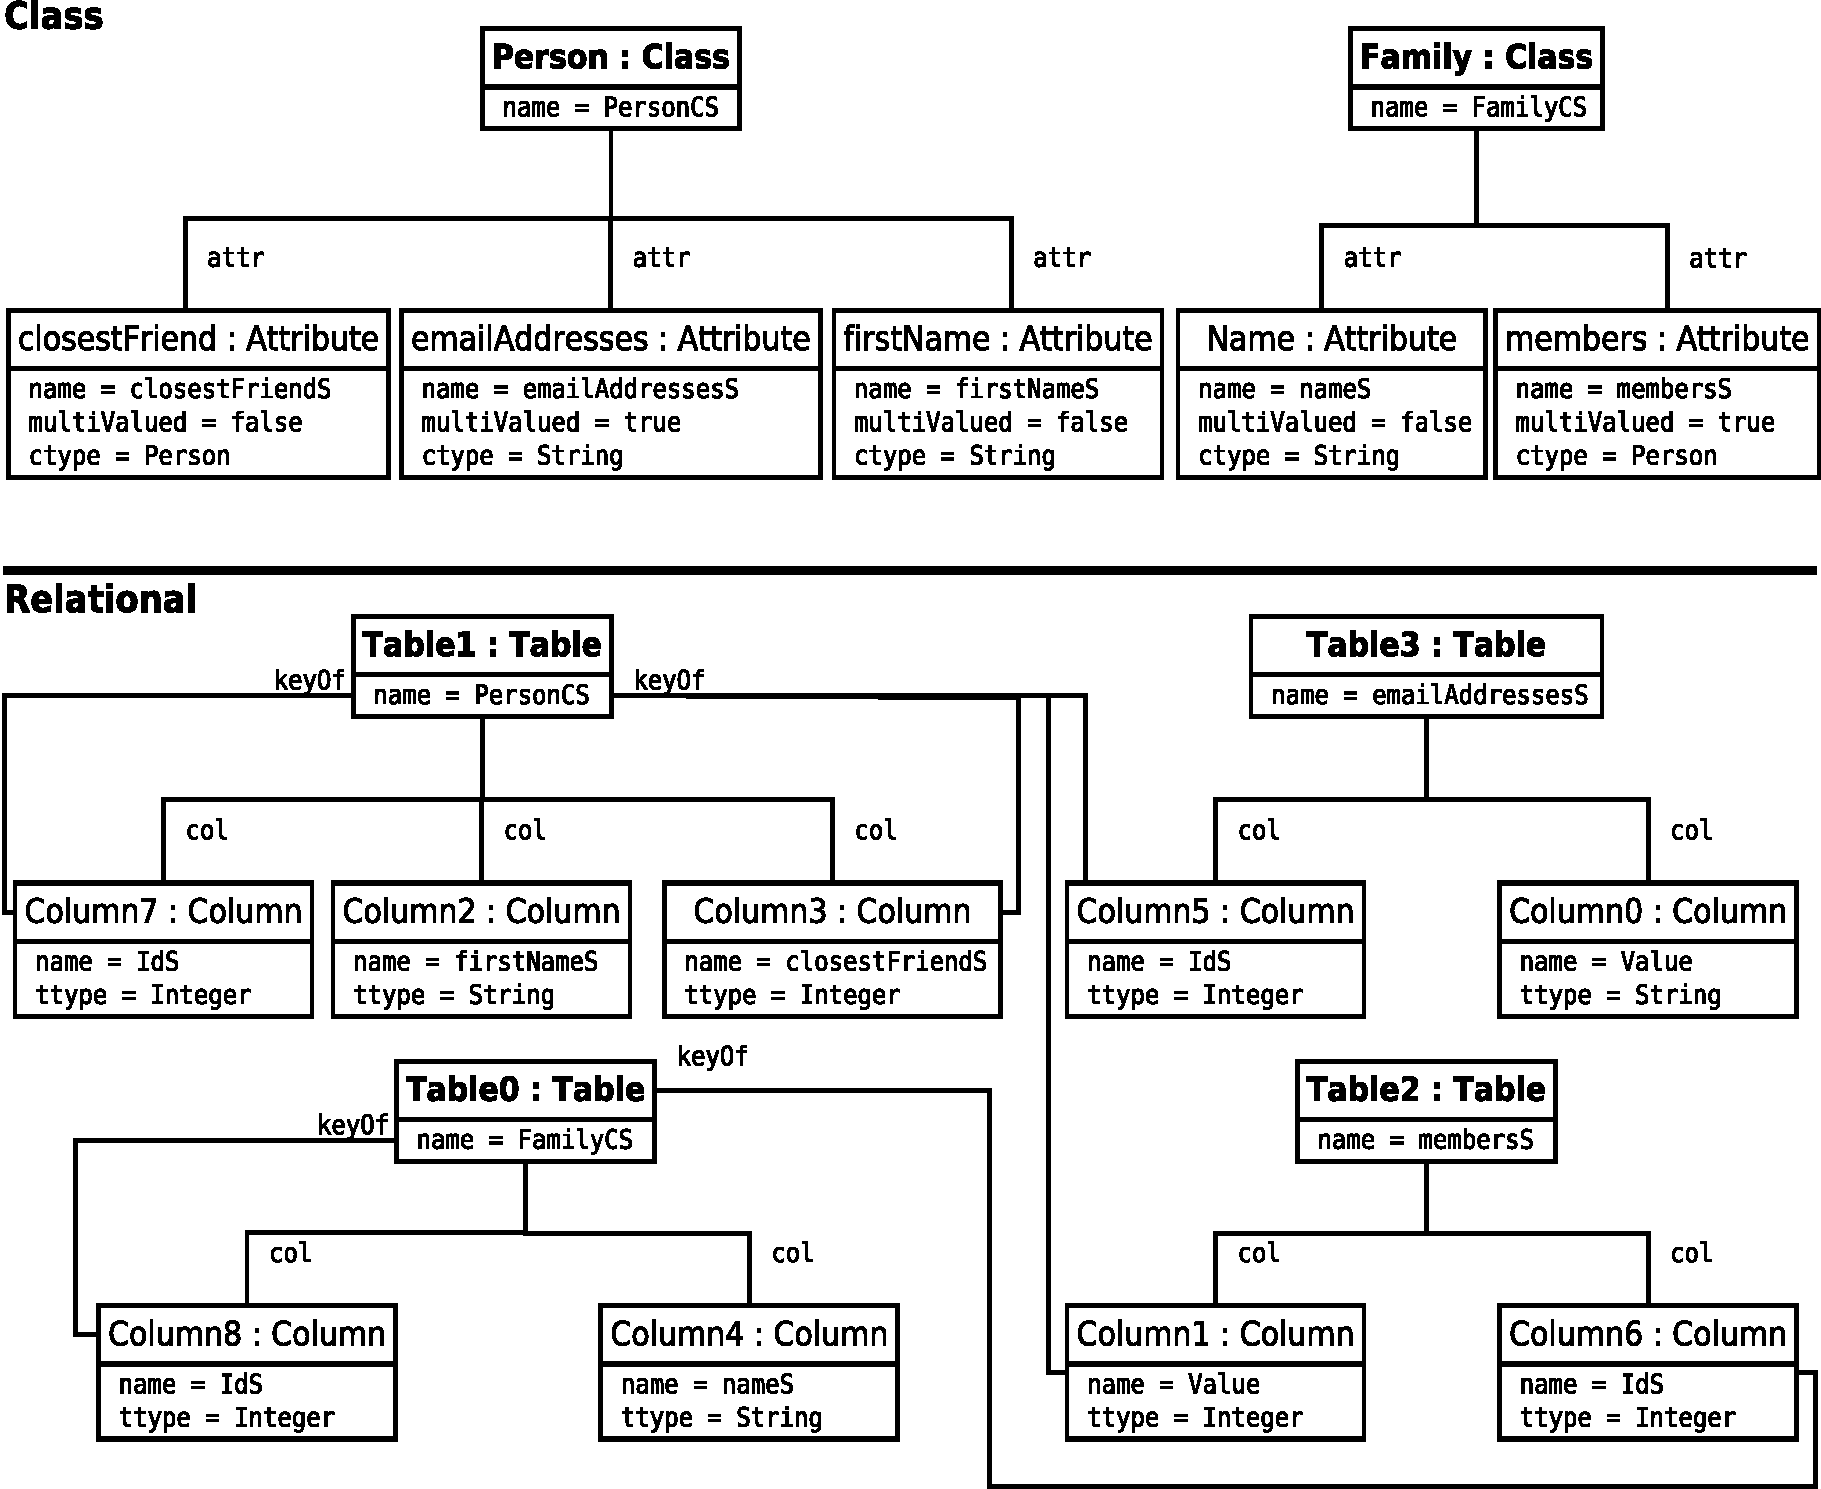
\includegraphics[scale=0.35]{img/diagram_scenario1.pdf}
\caption{Input and ouput from the running example (scenario 1) as instance diagrams}
\label{fig:transformation-result}
\end{figure}
%
From definition \ref{def:model-search}, a valid request must be a $partial$ $model$ of the transformation
metamodel ($CMM^T$). This property is ensured by the following proposition:
%
\begin{proposition} For all model $M^A$ that conformsTo $CMM^A$,
$M^A$ is a \emph{partial model} of (or p-$conformsTo$) $CMM^T$.
\end{proposition}
%
\begin{proof} From definition \ref{def:partial-model} of p-$conformsTo$, it
resolves to finding a relaxed metamodel $CMM^T_r = <MM^T_r,C^T_r> \in Rx(CMM^T)$ such that $M^A$ $conformsTo$ $CMM^T_r$. From definition \ref{def:conformance} of conformance, this requires that (1) $M^A$ $conformsTo$ $MM^T_r$ and (2) $M^A \in C(MM^T_r)$.\\
Let $CMM^T_r$ be the relaxed metamodel of $CMM^T$ such that $MM^T_r = MM^T$ and $C^T_r = \emptyset$ (i.e., the one obtained by removing all constraints). (2) is obviously true as there are no predicates to satisfy. (1) requires that $MM^T_r$ can be a reference model of $M^A$, i.e., its graph $G^T_r$ contains all nodes (meta-elements) targeted by the graph $G^A$ of $M^A$. This is clearly true since by definition \ref{def:transformation-metamodel} of $CMM^T$ we have $MM^A \subset MM^T$ (in particular $G^A \in G^T$), and on the other hand $MM^T_r = MM^T$ (in particular $G^T_r = G^T$).
\end{proof}

The second step is to perform the model search. This operation extends any model $M^A$ that conforms to $CMM^A$ into a model $M^T$ that conforms to $CMM^T$ (when there are solutions). By extending the source model, search produces a model $M^T$ which contains both the target elements and the weaving elements (these can be understood as the transformation traces). Additionally, model search ensures that the target elements satisfy their metamodel constraints, and optimization or preferences may be applied to discriminate between different solutions. To avoid adding source elements to the produced model, as usually expected in classical target creation scenarios, a set of model-level constraints can be added to $CMM^T$ in order to ``freeze'' the source model.\\
%
The final step is to isolate the target model $M^B$ that conforms to $CMM^B$. This can
easily be obtained by removing from $M^T$ any element that is not associated to $CMM^B$. In our example, a sample result is the ``Family" relational schema illustrated at the bottom of Figure \ref{fig:transformation-result}.
%
\subsection{Other scenarios}
%
The described scenario is a unidirectional one-to-one operation, but the approach is naturally bidirectional and can be used for different scenarios by varying the search request. Indeed, it suffices to use
$M^B$ as the request to obtain the reverse transformation (production of a model $M^A$). Additionally,
the synchronization scenario (propagating source or target model modifications to the
other one) can also be achieved with the same specifications: by using the union of the two models ($M^A$
and $M^B$) as the request, model search will extend them
to satisfy the transformation constraints, and thus update source,
target or both models (depending on the desired behaviour). Note that many CP solvers are restricted to constructive modifications since allowing for removal of elements from the request may yield tractability issues. However the approach itself does not prevent it and is only limited in this sense by the capabilities of the chosen underlying solver. All these scenarios are described and experimented on the running example in the next Section.\\
Finally, though these are not studied nor experimented in this paper, multi-source and/or multi-target transformations could also be achieved: it suffices to add the corresponding metamodels and weaving constraints to $CMM^T$, and corresponding models to the request. Indeed, constraints may have any arity (i.e., a single constraint may weave multiple metamodels elements).\\
In all these scenarios, the preceding propositions naturally hold as long as requests are partial models of $CMM^T$.
%
\section{Implementation and experiments}
\label{sec:validation}

In this section we first present the components used for implementing a prototype software chain. Second, we further describe the chosen use case and its realization on different scenarios. Finally, we summarize the experimentation results.

\subsection{Implementation}
%
The transformation as search (TAS) components were implemented using:
\begin{itemize}
\item the Eclipse Modeling Framework (EMF) \cite{ECORE} for defining, viewing and manipulating the various (meta)models presented in the preceding Section.
\item the ATL engine \cite{JouaultK05} for writing/executing the rule-based transformations of the process (unifying into $CMM^T$, projecting Ecore-OCL+ to/from the solver language, isolating the target model from the solution model).
\item Alloy/SAT \cite{DBLP:conf/sigsoft/Jackson00} as the constraint language/solver.
\end{itemize}
The software chain is freely available from a single package at \cite{TAS-CLAR-usecase}.

%
\subsection{Use case}
%
We have defined 3 scenarios:
\begin{enumerate} 
\item (1) the forward transformation presented in the running example (from class to relational)
\item (2) the reverse transformation (from relational to class)
\item (3) a synchronization scenario (propagation of changes from one model to another after adding new elements to the class schema). 
\end{enumerate}
The first goal was to experiment whether one single specification could handle different scenarios. The specification consists of a weaving metamodel, shown in the middle of Figure \ref{fig:classAndRelational}, which provides the basic correspondences between left and right metamodels. The figure shows correspondences between first-class elements (e.g., classes "Class" and "Table", classes "Attribute" and "Column", etc.). We defined a set of additional constraints, written in OCL+ (as illustrated in the code listing below), to further specify the weaving. Similarly to other transformation techniques, these specifications may be written in different ways. We provide results with two versions of the specifications, each of them used throughout all scenarios, to test the capabilities and behavior of the search. The first version (V1) mimics the behavior of the original (ATL) use case, in particular it creates simple integer columns for foreign keys. The second version (V2) has a more explicit (and better) handling of table primary/foreign keys. It also defines different weaving tables for each connected elements, allowing to write more specific constraints. Both versions can be found in package \cite{TAS-CLAR-usecase}.\\

As an example, the (V1) OCL+ excerpt below depicts 4 different kind of constraints attached to the weaving metamodel from Figure \ref{fig:classAndRelational}.\\
Constraint (1) specifies equality between the ``name" attribute of weaved ``Datatype" and ``Type" (similar constraints are given for ``Attribute", ``Class", ``Table" and ``Column").\\
Constraint (2) maps mono-valued attributes to columns (a similar constraint is given for multi-valued attributes/tables and classes/tables).\\
Constraint (3) ensures that weaved attributes/columns have a weaved datatype/type (a similar constraint handles classes and integer key columns).\\
Constraint (4) ensures that attributes cannot have both a weaved table and a weaved column (a similar constraint handles tables with classes and attributes).

\begin{verbatim}
1- context dtt : DataTypeAndType inv:
    dtt.wdatatype.name = dtt.wtype.name;
    
2- context att : Attribute inv:
    not att.multiValued implies att.caac.size() = 1;
    
3- context ac : AttributeAndColumn inv:
    ac.wattribute.ctype.oclIsTypeOf(DataType)
    and not ac.wattribute.multiValued
      implies ac.wcolumn.ttype = ac.wattribute.ctype.cdtat.wtype;
      
4- context att : Attribute inv:
    att.caac.size() + att.caat.size() = 1;
\end{verbatim}
%
%\newpage
%
\subsection{Experiments}
%
We experimented on the Family use case \cite{atlc2r}, which class schema is illustrated on the top of Figure \ref{fig:transformation-result}. This application is used as a proof-of-concept of our approach.The Alloy solver needs a specified pool of available elements: we set a maximum of 25 instances. We executed the model operations on an Intel Core Duo machine with 2.4GHz and 4GB of RAM. We used the Alloy Analyzer 4.2 with the MiniSat solver for generating search solutions. We summarize the results in Table \ref{tab:experiments-app1}. The given execution times correspond to the search of the first satisfying instance. They do not include the problem generation (projections from/to Ecore/Alloy, Alloy's compilation into SAT) since these are negligible in all our experiments and the metamodel projection only has to be done once for a given specification.\\
\begin{table}
\centering
\begin{tabular}{|c|c|c|c|c|}
\hline
scenario-version & \#variables & \#constraints & execution\\%& solver
 & (primary) & (unfolded) & time (ms)\\%&
\hline
\hline
(1) - V1 & 9956 & 845357 & 3432\\%& Alloy/MiniSAT
(1) - V2 & 7179 & 866894 & 2483\\
\hline
(2) - V1 & 10114 & 791167 & 5529\\%& Alloy/MiniSAT
(2) - V2 & 5725 & 866894 & 1655\\%& Alloy/MiniSAT
\hline
(3) - V1 & 6496 & 505227 & 324\\%& Alloy/MiniSAT
(3) - V2 & 5448 & 1231787 & 666\\%& Alloy/MiniSAT
\hline
\end{tabular}
\vspace{0.3cm}
\caption{Summary of the experiments (Family model)}
\label{tab:experiments-app1}
\end{table}

Alloy does not natively support strings as datatypes, we thus used predefined atoms and scalar equality (i.e., ``nameS" is the string ``name"). Both versions of the specifications generate the relational schema illustrated on the bottom of Figure \ref{fig:transformation-result}. However, if we cycle through the solutions, V1 also proposes solutions with additional ``orphan" tables. This can be prevented with a constraint that forbids creation of elements without a weaving association.\\
In the reverse transformation scenario (2), we used the exact generated target model (the Family table schema) as input request, freezing again the initial model through the pool of 25 available instances. Both versions generate the original class schema. However in V1, it is not the first found solution. Indeed, the first proposition is a class schema with an ``EmailAdresses" class (referenced by ``Person") and a ``Members" class (referenced by ``Family" and with an outgoing reference to ``Person"). This is a valid but nevertheless surprising solution at first. If desired, it is possible to prevent such behaviour with a weaving constraint that forces tables to become attributes whenever possible. This is done in V2 using the (explicit) table keys as conditions.\\
In the synchronization scenario (3), we used the whole transformation result from scenario 1 to create the input request: the class and relational schemas (as shown in Figure \ref{fig:transformation-result}), plus the generated weaving elements between them (transformation traces, not shown in the Figure). We then added to the class schema an ``Animal" class and its outgoing ``owner" reference to the ``Person" class. The goal was to test the propagation of changes to the table schema. Both versions update accordingly the relational schema, adding an ``Animal" table with an ``owner" (foreign) key column. The lower execution times are easily explained: search space is reduced since most of the model is given as input (only a limited number of SAT variables have to be assigned).
%
\subsection{Analysis and future work}
%
Experiments on these examples show that valid models can be created in different scenarios using single specifications, and that different solutions can be proposed to the designer. Although it is only a first step to assess the potential and flexibility of the approach, this prototype implementation can serve as a proof of feasibility. It is obvious that the produced models could already be obtained using existing transformation techniques, though this may require to write (or derive) additional specifications to handle all scenarios. Also, these experiments raise a number of modeling and operational challenges that will be considered in future work.\\
From the modeling point of view, defining specifications as weaving elements and constraints can be confusing for a designer used to traditional rule-based engines. For a given set of constraints, cycling through solutions or testing different scenarios may reveal a need to incrementally narrow some constraints, but also exhibit unexpected valid solutions. To ease the writing of specifications, a set of weaving templates can be provided as guidelines. Similarly, a mapping from a more specific language (such as QVT-relations \cite{QVT}) to an equivalent set of weaving templates can be studied. Also, additional scenarios can be considered. For instance, two independently-obtained models can be given to test (and exhibit) whether a valid mapping is able to relate them. The optimization/preferences capabilities of the approach are also to be experimented more deeply. Overall, an extensive evaluation on different sets of examples is necessary to confirm and exhibit the benefits that can be envisioned compared to existing techniques.\\
From the operational point of view, this prototype implementation will be extended and experiments conducted to assess tractability on larger models. Early experiments on a larger application, a graduate course management system extracted from a real-world system, show that the current Alloy-based implementation does not easily scale to medium-size models. The size of the instance pool is a major factor, and SAT compilation rapidly induces a combinatorial explosion in transformation scenarios (about 30000 variables and 10 minutes execution time). The propagation scenario seems more tractable (about 1 minute). Source and details of these experiments are also included in the package for reference. It is obvious that constraint solving is more (time) expensive than rule-based approaches (both theoretically and practically). However the constraint programming community has developped a large set of techniques to counter combinatorial explosion (structure-based symmetry breaking, decomposition, heuristics, etc.). The current implementation uses none of these.\\
Clearly, our aim is not to replace techniques that have proven suitable in many applications, but to show that the properties inherent to this approach are relevant for various problems, and how to integrate it in current MDE practices.
%
\section{Related work}
\label{sec:rfwork}
%
There are several approaches studying model transformations. A classification can be found at
\cite{czarnecki}. In particular, the OMG standard QVT \cite{QVT} has defined specifications for different type of model operations. Its QVT-operational part has been implemented by various tools such as the popular ATL \cite{JouaultK05}, TEFKAT \cite{tefkat}, VIATRA \cite{viatra}, and others. These approaches allow for fast and efficient unidirectional transformations. QVT-relations defines a broader set of capabilities, such as incremental transformations, but has fewer (and only partial) implementations such as \cite{Medini}.\\

Further studies have tackled bidirectional model transformations or synchronizations (see \cite{DBLP:conf/icmt/CzarneckiFHLST09} for a survey), often through mechanisms which require additional specifications to an existing rule-based transformation. For instance, \cite{DBLP:conf/icmt/HettelLR09} proposes, based on abductive reasoning, to reverse an unidirectional transformation in order to provide synchronization of the source model with the previously obtained target model. In particular, it shares our ability to compute different alternative solutions through combinatorial logic inference. A number of so-called incremental approaches \cite{DBLP:conf/models/HearndenLR06,DBLP:conf/models/VogelNHGB09,Bergmann:2008:IPM:1402947.1402953} allow to update a target model by taking into account incremental changes to the source model. Triple Graph Grammars (TGGs) \cite{tgg} are an approach for defining correspondences between two graphs. The TGG definition is similar to our model unification (i.e., a unique graph created from one left, one right and one correspondence graph) though not grounded in usual metamodelling principles. TGGs are also used for generating transformations (e.g., the \cite{fujaba} tool), but without search capabilities. \cite{DBLP:journals/sosym/AkehurstKP03,didonetphd} also expore the notion of weaving relationships but do not use them as direct transformation specifications. However, the described patterns may be useful in our context as specifications templates. Due to the high number of other existing transformation approaches and their spreading among different research communities, this overview can hardly be exhaustive. Clearly, many of these techniques have their own benefits over our approach, such as easier removal of elements or faster execution times. However, non-deterministic constrained search offers an original combination of properties: flexibility of having a single specification for different scenarios, ability to provide various solutions, automatic checking/optimizing capabilities, and in our case the sole use of existing modeling concepts.\\
%
Finally, the MDE community has also been using constraint-based solvers for various model operations
such as model checking \cite{DBLP:journals/scp/GogollaBR07,DBLP:conf/kbse/CabotCR07,DBLP:conf/splc/White1},
finding optimized transformations \cite{DBLP:conf/models/KessentiniSB08}, or extending transformation capabilities \cite{DBLP:conf/icmt/PetterBM09}. Although there are definitely similarities in the use of constraint tools, and in particular alternative mappings to solver languages, the pursued goals are different.
%
\section{Conclusion}
\label{sec:conclusion}
%
As model transformations have gained maturity in the past years, novel scenarios
have arised that cannot be handled using classical rule-based solutions, mainly
because of their non-deterministic nature. In this paper we described an original
approach in which the core idea is to \emph{search} for a solution model by
satisfying a set of weaving relations and constraints. The approach is built on a
previously defined operation, called model search, for the automatic generation
of complete valid models conforming to a metamodel and its constraints. Both
model search and transformation as search operations are based on the concepts of partial model and partial conformance.\\
The paper also describes how this model transformation technique is
formalized and automated as a first-class model operation, independently from
the solving engine, in order to fit in current MDE practices. The nature of the operation provides
original properties: bidirectionality, ability to explore and discriminate different target alternatives based on optimization criteria, synchronization of existing models, etc. However a larger set of examples and an extensive evaluation are required to assess practical benefits. Indeed, the provided prototype implementation on a reference usecase is only a first step that raises a number of modeling and operational challenges for future research.\\
%
\paragraph{Acknowledgements} this article was partially funded by project CNPq Universal (481715/2011-8) and Convênio Fundação Araucária/INRIA.
% %
%
% ---- Bibliography ----
%
\bibliography{18}
\bibliographystyle{plain}
%
\end{document}
